\documentclass[8pt,xcolor={dvipsnames}]{beamer}
\definecolor{MyBackground}{rgb}{1,1,1}
%\definecolor{MyBackground}{RGB}{190,190,190}
\setbeamercolor{background canvas}{bg=MyBackground}
\usetheme[
%%% option passed to the outer theme
%    progressstyle=fixedCircCnt,   % fixedCircCnt, movingCircCnt (moving is deault)
  ]{Feather}
  
% If you want to change the colors of the various elements in the theme, edit and uncomment the following lines

% Change the bar colors:
\setbeamercolor{Feather}{fg=NavyBlue!20,bg=NavyBlue}

% Change the color of the structural elements:
\setbeamercolor{structure}{fg=NavyBlue}

% Change the frame title text color:
\setbeamercolor{frametitle}{fg=black!5}

% Change the normal text colors:
\setbeamercolor{normal text}{fg=black!75,bg=gray!5}

%% Change the block title colors
\setbeamercolor{block title}{use=Feather,bg=Feather.fg, fg=black!90} 


% Change the logo in the upper right circle:
%\renewcommand{\logofile}{example-grid-100x100pt} 
%% This is an image that comes with the LaTeX installation
% Adjust scale of the logo w.r.t. the circle; default is 0.875
% \renewcommand{\logoscale}{0.55}

% Change the background image on the title and final page.
% It stretches to fill the entire frame!
% \renewcommand{\backgroundfile}{example-grid-100x100pt}

%-------------------------------------------------------
% INCLUDE PACKAGES
%-------------------------------------------------------

\usepackage[utf8]{inputenc}
\usepackage[english]{babel}
\usepackage{wrapfig}
\graphicspath{{Feathergraphics/}}
\let\latinencoding\relax
%\usepackage{fontspec}
\usepackage[T1]{fontenc}
% \usepackage{helvet}

%% Load different font packages to use different fonts
%% e.g. using Linux Libertine, Linux Biolinum and Inconsolata
% \usepackage{libertine}
% \usepackage{zi4}

%% e.g. using Carlito and Caladea
\usepackage{carlito}
\usepackage{caladea}
\usepackage{zi4}

%% e.g. using Venturis ADF Serif and Sans
% \usepackage{venturis}

%-------------------------------------------------------
% DEFFINING AND REDEFINING COMMANDS
%-------------------------------------------------------

% colored hyperlinks
\newcommand{\chref}[2]{
  \href{#1}{{\usebeamercolor[bg]{Feather}#2}}
}

%-------------------------------------------------------
% INFORMATION IN THE TITLE PAGE
%-------------------------------------------------------

\title[] % [] is optional - is placed on the bottom of the sidebar on every slide
{ % is placed on the title page
      \textbf{Wits Analytics and Visualization of Energy Systems}
}

\subtitle[Wits Analytics and Visualization of Energy Systems]
{
      \textbf{4\textsuperscript{th} Year Laboratory Project}
}

\author[Marion Heimann, Tristan Kuisis]
{      Marion Heimann, Tristan Kuisis 
}

\institute[]
{%
      School of Electrical and Information Engineering \\
      University of the Witwatersrand
}

\date{\today}

%-------------------------------------------------------
% THE BODY OF THE PRESENTATION
%-------------------------------------------------------

\begin{document}

%-------------------------------------------------------
% THE TITLEPAGE
%-------------------------------------------------------

{% % this is the name of the PDF file for the background
%\begin{frame}[plain,noframenumbering] % the plain option removes the header from the title page, noframenumbering removes the numbering of this frame only
 % \titlepage % call the title page information from above
%\end{frame}}

\begin{frame}{Project Overview}

%\begin{center}
%	
%	\begin{center}
%		\includegraphics[width=0.8\textwidth, trim=135 200 135 80, clip]{SystemOverviewGreen}
%	\end{center}
%\end{center}
%
%\small The project involves the use of multiple energy data loggers placed on the university campuses which record periodical energy use. Some of the dataloggers provide energy usage data as far back as 2013. The data obtained from the IST (ecWIN) system is manipulated and then imported into a time series database (OpenTSDB). A web framework is developed with the use of Flask.
%The web framework allows for the visualization of the data in a number of methods.
%The visualizations include:
%
%
%\begin{columns}
%	\begin{column}{0.5\textwidth}
%		\begin{itemize}
%			\item Time Series Line Charts (Dygraphs)
%			\item Heat Maps
%			\begin{itemize}
%				\item Colour Heat Map
%				\item Data Outage
%				\item Three Dimensional Heat Map
%			\end{itemize}
%			\item Sankey Diagram
%			\item Tree Map
%			\item Map
%			
%		\end{itemize}
%	\end{column}
%	\begin{column}{0.5\textwidth}  
%		\begin{center}
%			%%%%% this is a minipage, so \textwidth is already adjusted to the size of the column
%			
%			These visualizations allow for the unique interpretation of the day in multiple ways. Different visualization methods highlight different characteristics of the energy usage.
%		\end{center}
%	\end{column}
%\end{columns}


 The project involves the use of multiple energy data loggers placed on the university campuses which record periodical energy use. Some of the dataloggers provide energy usage data as far back as 2013. The data obtained from the IST (ecWIN) system is manipulated and then imported into a time series database (OpenTSDB). A web framework is developed with the use of Flask.
 
 \begin{wrapfigure}{l}{0.45\textwidth}
 	\begin{center}
 		\includegraphics[width=0.45\textwidth, trim=30 170 530 10, clip]{SystemOverviewGreenVertical}
 	\end{center}
 \end{wrapfigure}
The web framework allows for the visualization of the data in a number of methods.
The visualizations include:

\begin{itemize}
				\item Time Series Line Charts (Dygraphs)
				\item Heat Maps
				\begin{itemize}
					\item Colour Heat Map
					\item Data Outage
					\item Three Dimensional Heat Map
				\end{itemize}
				\item Sankey Diagram
				\item Tree Map
				\item Map
				
			\end{itemize}

These visualizations allow for the unique interpretation of the day in multiple ways. Different visualization methods highlight different characteristics of the energy usage.
\end{frame}


\begin{frame}{Database}
%\begin{block}{OpenTSDB}

\begin{wrapfigure}{l}{0.39\textwidth}
	\begin{center}
		\includegraphics[width=0.38\textwidth, trim=65 80 450 60, clip]{OpenTSDBNo}
	\end{center}
\end{wrapfigure}

Time series database (TSDB) is inherently useful for this type of data as it makes use of key-value pairs. These key value pairs are made up of a timestamp and a corresponding energy usage value for a specific time period.
The database has a convenient set of utilities that allow for importing, managing, and querying the required data. OpenTSDB is made up of a Time Series Daemon (TSD) which allows users to interact with underlying data. This is stored using Apache HBase or Google Bigtable.
These provide a distributed and  highly scalable data storage solution.
Interaction with the data is done using number of supported methods: a telnet-style protocol, an HTTP API, or the built in user interface.

%\vspace{5mm}
%%\begin{block}{Writing to the Database}
%	\textbf{Writing to the Database}

\begin{exampleblock}{Writing to the Database}
	
	\small Metrics have been used as the major identifiers of the different data loggers and their readings, tags are used to affix additional information to the data points.
	
	\begin{center}
		\includegraphics[width=0.98\textwidth, trim=13 210 15 180, clip]{WritingToTheDatabaseNotBold}
	\end{center}
\end{exampleblock}
	
%\end{block}
	
	
%\end{block}

\end{frame}

%\begin{frame}{Database}
%
%\begin{block}{Writing to Database}
%
%Writing data to the database can be done using three methods: Telnet, an HTTP API, or internel OpenTSDB importing tools.
%Each time series point is imported into the database and each component of the data specification is important for querying ability further down the line. Metrics have been used as the major identifiers of the different data loggers and their readings, tags are important to identify cases where data outages occurred. The use of tags is highly relevant when extra information can be affixed to specific data points in time. This can be in cases where a unique data outage occurred or an abnormal reading was taken and an explanation is required.
%	\begin{center}
%		\includegraphics[width=0.98\textwidth, trim=13 210 15 180, clip]{WritingToTheDatabaseNotBold}
%	\end{center}
%\end{block}
%
%\end{frame}


\begin{frame}{Web Framework}{Flask Server}

\begin{columns}
	\begin{column}{0.4\textwidth}
		
		The web framework is used to provide processing for visuals and a front end. The flask framework, in conjunction with the Python requests package allows for easily querying the OpenTSDB database.
		Flask makes use of the Jinja2 templating engine (within Python), which allows for the use of static web pages to be reused while creating dynamic content.
		The web server allows for short feedback cycles (testing) on the developers local machine. The web server can easily be ported to a more permanent solution on a dedicated server.
		
	\end{column}
	\begin{column}{0.6\textwidth}  
			\begin{center}
			\includegraphics[width=\textwidth, trim=0 0 490 30, clip]{FlaskDiagram}
		\end{center}
	\end{column}
\end{columns}

%\begin{wrapfigure}{r}{0.55\textwidth}
%	\begin{center}
%		\includegraphics[width=0.55\textwidth, trim=0 0 490 30, clip]{FlaskDiagram}
%	\end{center}
%\end{wrapfigure}
%
%The web framework is used to provide processing for visuals and a front end. The flask framework, in conjunction with the Python requests package allows for easily querying the OpenTSDB database.
%Flask makes use of the Jinja2 templating engine (within Python), which allows for the use of static web pages to be reused while creating dynamic content.
%The web server allows for short feedback cycles (testing) on the developers local machine. The web server can easily be ported to a more permanent solution on a dedicated server.

\end{frame}

%\begin{frame}{Dataloggers and IST}
%IST's product, ecWIN, is employed on the universities campuses such that there is a central point where the energy readings can be accumulated and managed. This system allows for the monitoring of energy usage from the data loggers installed throughout the campuses.
%This web portal has been used to draw the historical data from the data loggers, some of which go back to 2013.
%\end{frame}

\begin{frame}{Dygraphs}

Simple, interactive visualisation of the energy usage. It can highlight patterns, and anomalies within the data. This is highly relevant in cases where the validity of the data is in question.
	\begin{center}
		\includegraphics[width=\textwidth, trim=0 0 0 0, clip]{DygraphsJubilee2014_2018}
	\end{center}
\end{frame}

\begin{frame}{Heatmap}

%Colour representation of relative magnitudes of energy is created with the use of block corresponding to hours in the day. 
%Colour representation of relative magnitudes of energy is shown. 
Each block represents a time of day (y-axis), the date (x-axis) and the relative magnitude of energy (colour intensity and hue).
This is particularly useful for illustrating trends over large regions of time. 

% Zoomed out Jubilee Hall
\begin{center}
	\includegraphics[width=\textwidth, trim=30 50 70 50, clip]{HeatMapCollegeHouse}
\end{center}
\end{frame}


\begin{frame}{Data Outage Visualisation}
Each block represents a time of day (y-axis), the date (x-axis) and the relative magnitude of energy (colour: black or white).
This is particularly useful for highlighting data outages by strongly contrasting the points with data and those without. 

% Zoomed out Jubilee Hall
\begin{center}
	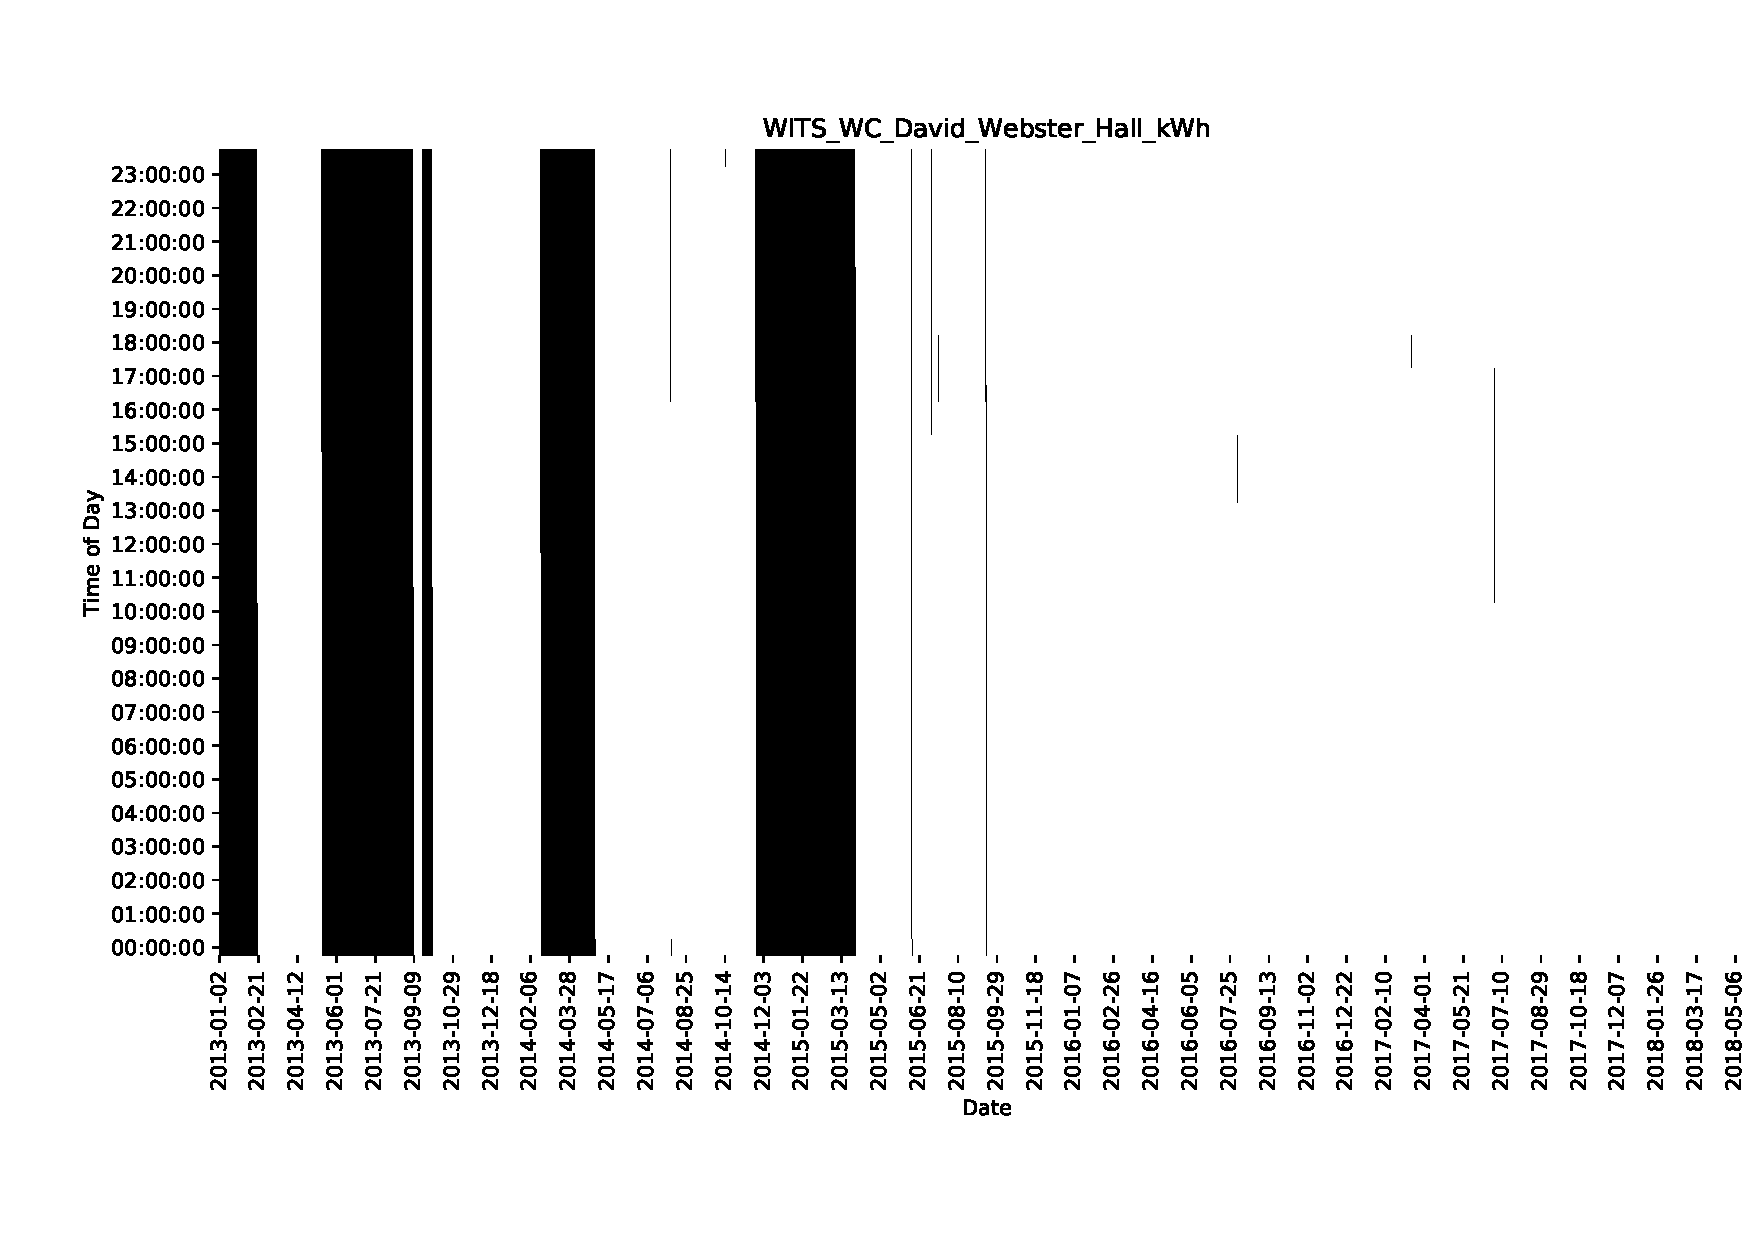
\includegraphics[width=\textwidth, trim=30 30 0 50, clip]{DataOutageDavidWebster}
\end{center}
\end{frame}


\begin{frame}{Sankey Diagram}

The widths of each of the bands are proportional to the energy incoming, and consumption through the system. The ability to visually compare the widths with reference to eachother provides reference points of magnitudes. 
This can effectively highlight unnaccounted for energy within the system, which can be the case where portions of the system are unmetered.
\begin{center}
	\includegraphics[width=\textwidth, trim=20 10 130 0, clip]{SankeyMatrix}
\end{center}
\end{frame}


\begin{frame}{Treemap}
A display of the hierarchical nature of the data. The sizes of the geometrical shapes indicate the relative energy of the chosen meters. This is useful to identify the major energy consumers.
% Zoomed out Jubilee Hall
\begin{center}
	\includegraphics[width=\textwidth, trim=0 0 0 10, clip]{Treemap}
\end{center}
\end{frame}


\begin{frame}{Choropleth Map}

This visualization provides user with the geographical representation of the energy use of specific areas. This is particularly useful when building names are not known and to compare the energy usage in various buildings.

	\begin{center}
		\includegraphics[width=0.68\textwidth, trim=0 0 0 0, clip]{ChoroplethMap}
	\end{center}


% Zoomed out Jubilee Hall
%\begin{center}
%	\includegraphics[width=0.7\textwidth, trim=0 2 0 0, clip]{ChoroplethMap}
%\end{center}
\end{frame}
%
%\begin{frame}{Content}{}
%\tableofcontents
%\end{frame}
%
%%-------------------------------------------------------
%\section{Introduction}
%%-------------------------------------------------------
%\subsection{License}
%\begin{frame}{Introduction}{License}
%%-------------------------------------------------------
%
%  \begin{itemize}
%    \item<1-> The Feather image is not covered by copyright rules. I have used the image from \chref{http://www.vectors-free.com/}{http://www.vectors-free.com/}. You are allowed to use the Feather image for any purposes.
%    \item<2-> The rest of the theme is provided under the GNU General Public License v. 3 (GPLv3) \chref{http://www.gnu.org/licenses/}{http://www.gnu.org/licenses/}. This means that you can redistribute it and/or modify it under the same license. 
%  \end{itemize}
%\end{frame}
%
%%-------------------------------------------------------
%\section{Installation}
%%-------------------------------------------------------
%\subsection{Source files}
%\begin{frame}{Installation}{Source files}
%%-------------------------------------------------------
%
%\begin{block}{}
%The theme contains 4 source files:
%  \begin{itemize}
%    \item {\tt beamercolorthemeFeather.sty}
%    \item {\tt beamerouterthemeFeather.sty}
%    \item {\tt beamerinnerthemeFeather.sty}
%    \item {\tt beamerthemeFeather.sty}
%  \end{itemize}
%\end{block}
%\end{frame}
%
%%-------------------------------------------------------
%\subsection{Local and Global installation}
%\begin{frame}{Installation}{Local and Global installation}
%%-------------------------------------------------------
%  The theme can be installed for \textbf{local} or \textbf{global} use.
%  \pause
%  \begin{block}{Local Installation}
%  \begin{itemize}    
%    \item Local installation is the simplest way of installing the theme. 
%    \item You need to placing the 4 source files in the same folder as your presentation. When you download the theme, the 4 theme files are located in the {\tt local} folder.
%  \end{itemize}
%  \end{block}
%
%  \begin{block}{Global Installation}
%  \begin{itemize}
%     \item If you wish to make the theme globally available, you must put the files in your local latex directory tree. The location of the root of the local directory tree depends on your operating system and the latex distribution. 
%     \item Detailed steps on how to proceed installation under various operating systems can be found at Beamer documentation.
%  \end{itemize}
%  \end{block}
%\end{frame}
%     
%
%%-------------------------------------------------------
%\subsection{Required Packages}
%\begin{frame}{Installation}{Required Packages}
%%-------------------------------------------------------
%
%  For using the Feather Theme you will need the Bemaer class installed and the following 2 packages
%  \begin{itemize}
%    \item TikZ\footnote{TikZ is a package for creating beautiful graphics. Have a look at these \chref{http://www.texample.net/tikz/examples/}{online examples} or the \chref{http://tug.ctan.org/tex-archive/graphics/pgf/base/doc/generic/pgf/pgfmanual.pdf}{pgf user manual}.}
%    \item calc
%  \end{itemize}
%  Due to the fact that the packages are very common they should be included in your latex distribution in the first place.
%\end{frame}
%
%%-------------------------------------------------------
%\section{User Interface}
%\subsection{Loading the Theme and Theme Options}
%\begin{frame}{User Interface}{Loading the Theme and Theme Options}
%%-------------------------------------------------------
%
%  \begin{block}{The Presentation Theme}
%    The Feather Theme can be loaded in a familiar way. In the reamble of your {\tt tex} file you must type\\ \vspace{5pt} 
%    {\tt \textbackslash usetheme[<options>]\{Feather\}}\\ \vspace{5pt} 
%    The presentation theme loads the inner, outer and color Feather theme files and passes the {\tt <options>} on to these files.
%  \end{block}
%  \begin{block}{The Inner and Outher Themes}
%    If you wish you can load only the inner, or the outher theme directly by\\ \vspace{5pt} 
%    {\tt \textbackslash useinnertheme\{Feather\}} (and it has no options)\\ \vspace{5pt} 
%    {\tt \textbackslash useoutertheme[<options>]\{Feather\}} (it has one option)\\
%    \hspace{20pt}{\tt progressstyle=\{fixedCircCnt or movingCircCnt\}} \\
%    \begin{itemize}
%    \item which set how the progress is illustrated;
%    \item the value {\tt movingCircCnt} is the default.
%    \end{itemize}
%  \end{block}
%\end{frame}
%
%\begin{frame}{User Interface}{Loading the Theme and Theme Options}
%
%  \begin{block}{The Color Theme}
%    Also you can load only the color theme by writing in the preamble of the {\tt tex} file 
%    
%    \vspace{5pt} 
%    
%    \begin{itemize}
%    \item {\tt \textbackslash usecolortheme\{Feather\}}
%    \end{itemize}
%    
%    \vspace{5pt}
%    
%    ...or to change the colors of the various elements in the theme
%    
%    \vspace{5pt} 
%    \begin{itemize}
%    \item Change the bar colors: \\    
%    {\tt \textbackslash setbeamercolor \{Feather\}\{fg=<color>, bg=<color>\}}
%    
%    \vspace{2pt} 
%    
%    \item Change the color of the structural elements: \\    
%    {\tt \textbackslash setbeamercolor\{structure\}\{fg=<color>\}}
%    
%    \vspace{2pt} 
%    
%    \item Change the frame title text color:\\
%    {\tt \textbackslash setbeamercolor\{frametitle\}\{fg=<color>\}}
%    
%    \vspace{2pt} 
%    
%    \item Change the normal text color background:    
%    {\tt \textbackslash setbeamercolor\{normal text\}\{fg=<color>, bg=<color>\}}
%    \end{itemize}
%  \end{block}
%\end{frame}
%
%
%%-------------------------------------------------------
%\subsection{Feather image}
%\begin{frame}{User Interface}{The Feather Background Image}
%%-------------------------------------------------------
%
%\begin{block}{The Feather Background Image}
%    \begin{itemize}
%    \item In Feather theme, the title page frame and the last frame have the Feather image as the background image. 
%    \item The Feather background image can be produced to any frame by wrating on the begining at the choosen frame the following
%    \end{itemize} 
%    
%    \vspace{5pt} 
%    
%  {\tt \{\textbackslash 1bg\\
%    \textbackslash begin\{frame\}[<options>]\{Frame Title\}\{Frame Subtitle\}\\
%    \ldots\\
%    \textbackslash end\{frame\}\}}
%\end{block}
%\end{frame}
%
%
%{
%\begin{frame}[plain,noframenumbering]
%  \finalpage{Thank you for using Feather Beamer Theme!}
%\end{frame}}

\end{document}